
\documentclass[12pt]{article}
\usepackage{amsfonts}

%%%%%%%%%%%%%%%%%%%%%%%%%%%%%%%%%%%%%%%%%%%%%%%%%%%%%%%%%%%%%%%%%%%%%%%%%%%%%%%%%%%%%%%%%%%%%%%%%%%
\usepackage{amsmath,amssymb,amsthm}
\usepackage{multicol}
\usepackage{color}
\usepackage{hyperref}
\usepackage{graphicx}
\usepackage[english]{babel}

%TCIDATA{OutputFilter=Latex.dll}
%TCIDATA{LastRevised=Mon Oct 10 18:16:16 2011}
%TCIDATA{<META NAME="GraphicsSave" CONTENT="32">}
%TCIDATA{CSTFile=article.cst}

\newtheorem{Def}{Definition}[section]
\newtheorem{Cnj}[Def]{Conjecture}
\newtheorem{Prop}[Def]{Property}
\newtheorem{example}{Example}[section]

%\input{tcilatex}

\begin{document}
\title{Fan, splint and branching rules.}



\author{V.D.~Lyakhovsky$^1$, A.A.~Nazarov$^{1,2}$ \\
  {\small $^1$ Department of High-energy and elementary particle physics, SPb State University}\\
  {\small 198904, Saint-Petersburg, Russia}\\
  {\small e-mail: lyakh1507@nm.ru}\\
  {\small$^{2}$ Chebyshev Laboratory,}\\
  {\small Department of Mathematics and Mechanics, SPb State University}\\
  {\small 199178, Saint-Petersburg, Russia}\\
  {\small email: antonnaz@gmail.com}}
\maketitle

\begin{abstract}
Splint of root system of simple Lie algebra appears naturally in
the study of (regular) embeddings of reductive subalgebras. It can
be used to derive branching rules. We show that application of
splint properties drastically simplifies calculations of
branching coefficients.
\end{abstract}

\section{Introduction}
\label{sec:Introduction}

Splint $\phi$ of a root system $\Delta_1$ into a root system
$\Delta$ is a bijective map of roots of $\Delta_{1}$ to (proper)
subset of $\Delta$ which commutes with vector composition law in
$\Delta_{1}$ and $\Delta$.
\begin{equation*}
\phi:\Delta_1 \longrightarrow \Delta
\end{equation*}
\begin{equation*}
\phi \circ (\alpha + \beta) =\phi \circ \alpha + \phi \circ \beta,
\,\,\, \alpha,\beta \in \Delta_1
\end{equation*}

Note that the image $Im(\phi)$ must not inherit the root system
properties except the addition rules equivalent to the addition
rules in $\Delta_{1}$ (for pre-images). The term {\it splint} was
introduced by D. Richter in  \cite{richter2008splints} where the
classification of splints for simple Lie algebras was obtained.
There was also mentioned that the notion of splint must have tight
connections with the injection fan approach. The fan $\Gamma
\subset \Delta$ was
introduced in \cite{lyakhovsky1996rra} as the subset of root system describing recurrent
properties of branching coefficients for maximal embeddings  . Injection fan is an
efficient tool to study branching rules. Later this construction
was generalized to non-maximal embeddings and infinite-dimensional
Lie algebras in \cite{2010arXiv1007.0318L, ilyin812pbc}.

In the present paper we study the connection of splint with
injection fan for regular embeddings of reductive subalgebras
${\mathfrak a}\longrightarrow {\mathfrak g}$. We show that (under
certain conditions described in section \ref{sec:stems and
multiplicity functions}) splint is a natural tool to study
reduction properties of simple Lie algebra ${\mathfrak g}$-modules
with respect to a subalgebra ${\mathfrak a}\longrightarrow
{\mathfrak g}$. Using this tool we obtain the main result of the
present paper -- the one-to-one correspondence between weight
multiplicities in irreducible modules of splint and branching
coefficients for a reduced module $L^{\mu}_{{\mathfrak
g}\downarrow {\mathfrak a}}$.


\section{Injections and splints}

\label{sec:Injections and splints}

Consider a simple Lie algebra $\mathfrak{g}$ and its regular subalgebra $%
\mathfrak{a}\longrightarrow \mathfrak{g}$ such that $\mathfrak{a}$
is a
reductive subalgebra $\mathfrak{a \subset g}$ with correlated root spaces: $%
\mathfrak{h}_{\mathfrak{a}}^{\ast }\subset \mathfrak{h}_{\mathfrak{g }%
}^{\ast }$. Let $\mathfrak{a}^S$ be a semisimple summand of
$\mathfrak{a}$,
this means that $\mathfrak{a}=\mathfrak{a}^S \oplus \mathfrak{u}(1)\oplus %
\mathfrak{u}(1)\oplus \dots$. We shall consider $\mathfrak{a}^S$
to be a proper regular subalgebra and $\mathfrak{a}$ to be the
maximal subalgebra with $\mathfrak{a}^S$ fixed that is the rank
$r$ of $\frak{a}$ is equal to that of $\mathfrak{g}$.

$r$ , $\left( r_{\mathfrak{a}^S}\right) $ --- the rank of
$\frak{g}$ $\left( \mathrm{{resp. }\mathfrak{a}^S}\right) $ ;

$\Delta $ $\left( \Delta _{\frak{a}}\right) $--- the root system;
$\Delta ^{+} $ $\left( \mathrm{{resp. }\Delta
_{\frak{a}}^{+}}\right) $--- the positive root system (of
$\frak{g}$ and $\frak{a}$ respectively);

$S\quad \left( S_{\frak{a}}\right) $ --- the system of simple roots (of $%
\frak{g}$ and $\frak{a}$ respectively);

$\alpha _{i}$ , $\left( \alpha _{\left( \frak{a}\right) j}\right) $ --- the $%
i$-th (resp. $j$-th) simple root for $\frak{g}$ $\left( \mathrm{{resp.}\frak{%
a}}\right) $; $i=0,\ldots ,r$,\ \ $\left( j=0,\ldots ,r_{\mathfrak{a}%
^S}\right) $;

$W$ , $\left( W_{\frak{a}}\right) $--- the corresponding Weyl group;

$C$ , $\left( C_{\frak{a}}\right) $--- the fundamental Weyl chamber;

$\bar{C}, \left(\bar{C_{\frak{a}}}\right)$ --- the closure of the
fundamental Weyl chamber;

$\epsilon \left( w\right) :=\left( -1\right) ^{\mathrm{length}(w)}$;

$\rho $\ , $\left( \rho _{\frak{a}}\right) $\ --- the Weyl vector;

$L^{\mu }$\ $\left( L_{\frak{a}}^{\nu }\right) $\ --- the integrable module
of $\frak{g}$ with the highest weight $\mu $\ ; (resp. integrable $\frak{a}$
-module with the highest weight $\nu $ );

$\mathcal{N}^{\mu }$ , $\left( \mathcal{N}_{\frak{a}}^{\nu }\right) $ ---
the weight diagram of $L^{\mu }$ (resp. ${}L_{\frak{a}}^{\nu }$ );

$P$ (resp. $P_{\frak{a}} $) \ --- the weight lattice;

$P^{+}$ (resp. $P_{\frak{a}}^{+} $) \ --- the dominant weight lattice;

$\mathcal{E}$ (resp. $\mathcal{E}_{\frak{a}} $) \ --- the formal algebra;

$m_{\xi }^{\left( \mu \right) }$ , $\left( m_{\xi }^{\left( \nu \right)
}\right) $ --- the multiplicity of the weight $\xi \in P$ \ $\left( \mathrm{{%
resp. }\in P_{\frak{a}}}\right) $ in the module $L^{\mu }$ , (resp. $\xi \in
L_{\frak{a}}^{\nu } $);

$ch\left( L^{\mu }\right) $ (resp. $\mathrm{ch}\left( L_{\frak{a}}^{\nu
}\right) $)--- the formal character of $L^{\mu }$ (resp. $L_{\frak{a}}^{\nu
} $);

$ch\left( L^{\mu }\right)  =\frac{\sum_{w\in W}\epsilon (w)e^{w\circ (\mu
+\rho )-\rho }} {\prod_{\alpha \in \Delta ^{+}} \left( 1-e^{-\alpha }\right)
} $ --- the Weyl formula;

$R:=\prod_{\alpha \in \Delta ^{+}}\left( 1-e^{-\alpha }\right) \quad $
(resp. $R_{\frak{a}}: =\prod_{\alpha \in \Delta_{\frak{a}}^{+}} \left(
1-e^{-\alpha }\right) $ ) --- the Weyl denominator.

Let $L^{\mu }$ be completely reducible with respect to $\frak{a}$,
\[
L_{\frak{g}\downarrow \frak{a}}^{\mu }=\bigoplus\limits_{\nu \in P_{\frak{a}%
}^{+}}b_{\nu }^{\left( \mu \right) }L_{\frak{a}}^{\nu }.
\]
\begin{equation}
\pi _{\frak{a}}ch\left( L^{\mu }\right) =\sum_{\nu \in P_{\frak{a}%
}^{+}}b_{\nu }^{(\mu )}ch\left( L_{\frak{a}}^{\nu }\right) .
\label{branching1}
\end{equation}
For the modules we are interested in the Weyl formula for $\mathrm{ch}\left(
L^{\mu }\right) $ can be written in terms of singular elements \cite
{humphreys1997introduction}
\[
\Psi ^{\left( \mu \right) }:=\sum\limits_{w\in W}\epsilon (w)e^{w(\mu +\rho
)-\rho },
\]
namely,
\begin{equation}
\mathrm{ch}\left( L^{\mu }\right) =\frac{\Psi ^{\left( \mu \right) }}{\Psi
^{\left( 0\right) }}=\frac{\Psi ^{\left( \mu \right) }}{R}.
\label{Weyl-Kac2}
\end{equation}
The same is true for submodules $\mathrm{ch}\left( L_{\frak{a}}^{\nu
}\right) $ in (\ref{branching1})
\[
\mathrm{ch}\left( L_{\frak{a}}^{\nu }\right) =\frac{\Psi _{\frak{a}}^{\left(
\nu \right) }}{\Psi _{\frak{a}}^{\left( 0\right) }}=\frac{\Psi _{\frak{a}%
}^{\left( \nu \right) }}{R_{\frak{a}}},
\]
with
\[
\Psi _{\frak{a}}^{\left( \nu \right) }:=\sum\limits_{w\in W_{\frak{a}%
}}\epsilon (w)e^{w(\nu +\rho _{_{\frak{a}}})-\rho _{_{\frak{a}}}}.
\]

Applying formula (\ref{Weyl-Kac2}) to the branching rule (\ref{branching1})
we get the relation connecting the singular elements $\Psi ^{\left( \mu
\right) }$ and $\Psi _{\frak{a}}^{\left( \nu \right) }$ :
\begin{eqnarray}
\frac{\sum_{w \in W}\epsilon (w )e^{w (\mu +\rho )-\rho }}{\prod_{\alpha \in
\Delta ^{+}}(1-e^{-\alpha })} &=&\sum_{\nu \in P_{\frak{a}}^{+}}b_{\nu
}^{(\mu )}\frac{\sum_{w \in W_{\frak{a}}}\epsilon (w )e^{w (\nu +\rho _{%
\frak{a}})-\rho _{\frak{a}}}}{\prod_{\beta \in \Delta _{\frak{a}%
}^{+}}(1-e^{-\beta })},  \nonumber  \label{eq:4} \\
\frac{\Psi ^{\left( \mu \right) }}{R} &=&\sum_{\nu \in P_{\frak{a}%
}^{+}}b_{\nu }^{(\mu )}\frac{\Psi _{\frak{a}}^{\left( \nu \right) }}{R_{%
\frak{a}}}.  \label{singular main}
\end{eqnarray}

In \cite{2010arXiv1007.0318L} it was proven that branching coefficients $%
b_{\xi }^{\left( \mu \right) }$ corresponding to the injection $\frak{a}%
\hookrightarrow \frak{g}$ are subject to the set of recurrent relations:
\begin{equation}
\begin{array}{c}
b_{\xi }^{\left( \mu \right) }=-\frac{1}{s\left( \gamma _{0}\right) }\left(
\sum_{u\in U}\epsilon (u)\;\dim \left( L_{\frak{a}_{\perp }}^{\mu _{\frak{a}%
_{\perp }}\left( u\right) }\right) \delta _{\xi -\gamma _{0},\pi _{%
\widetilde{\frak{a}}}(u(\mu +\rho )-\rho )}+\right. \\
\left. +\sum_{\gamma \in \Gamma _{\widetilde{\frak{a}}\rightarrow \frak{g}%
}}s\left( \gamma +\gamma _{0}\right) b_{\xi +\gamma }^{\left( \mu \right)
}\right) .
\end{array}
\label{recurrent rel}
\end{equation}
where $\frak{a}_{\perp }$ is the subalgebra determined by the roots of $%
\frak{g}$ orthogonal to roots of $\frak{a}$
\begin{eqnarray}
\Delta _{\frak{a}_{\perp }} &:&=\left\{ \beta \in \Delta _{\frak{g}}|\forall
h\in \frak{h}_{\frak{a}};\beta \left( h\right) =0\right\} ,
\label{delta a ort}
\end{eqnarray}
\begin{eqnarray}
\widetilde{\frak{a}_{\perp }} :=\frak{a}_{\perp }\oplus \frak{h}_{\perp }
\qquad \widetilde{\frak{a}} :=\frak{a}\oplus \frak{h}_{\perp }
\end{eqnarray}
and $\pi$ is the projection operator. When the injection is maximal the
projection becomes trivial and the relation (\ref{recurrent rel}) is
simplified:
\begin{equation}
\begin{array}{c}
b_{\xi }^{\left( \mu \right) }=-\frac{1}{s\left( \gamma _{0}\right) }\left(
\sum_{u\in W}\epsilon (u) \delta _{\xi -\gamma _{0}, u(\mu +\rho )-\rho
}+\right. \\
\left. +\sum_{\gamma \in \Gamma _{\frak{a}\rightarrow \frak{g}}}s\left(
\gamma +\gamma _{0}\right) b_{\xi +\gamma }^{\left( \mu \right) }\right) .
\end{array}
\label{recurrent relation max}
\end{equation}
The recursion is goverened by the set $\Gamma _{\frak{a}\rightarrow \frak{g}}
$ called the injection fan. The latter is defined by the carrier set $%
\left\{ \xi \right\} _{\frak{a}\rightarrow \frak{g}}$ for the coefficient
function $s(\xi )$
\[
\left\{ \xi \right\} _{\frak{a}\rightarrow \frak{g}}:=\left\{ \xi \in P_{%
\frak{a}}|s(\xi )\neq 0\right\}
\]
appearing in the expansion
\begin{equation}
\prod_{\alpha \in \Delta ^{+}\setminus \Delta _{\frak{a}}^{+}}\left( 1-e^{
-\alpha }\right) =-\sum_{\gamma \in P_{\frak{a}}}s(\gamma )e^{-\gamma };\quad
\label{product}
\end{equation}

Now we remind two definitions introduced in \cite{richter2008splints}

\begin{Def}
Suppose $\Delta _{0}$ and $\Delta $ are root systems with the corresponding
weight lattices $P_{0}$ and $P$. Then $\phi $ is an ``embedding'',
\begin{equation}
\phi :\left\{
\begin{array}{l}
\Delta _{0}\hookrightarrow \Delta , \\
P_{0}\hookrightarrow P,
\end{array}
\right.
\end{equation}
if \newline
\noindent (a) it injects $\Delta _{0}$ in $\Delta $, and \newline
\noindent (b) acts homomorphically with respect to the vector groups in $%
P_{0}$ and $P$:
\[
\phi (\gamma )=\phi (\alpha )+\phi (\beta )
\]
for any triple $\alpha ,\beta ,\gamma \in P_{0}$ such that $\gamma =\alpha
+\beta $.
\end{Def}

$\phi$ induces an injection of formal algebras $:{\mathcal{E}}_0
\longrightarrow \mathcal{E}$ and for the image ${\mathcal{E}}%
_i=Im_{\phi}\left( {\mathcal{E}}_0\right)$ one can consider its inverse $%
\phi^{-1}:{\mathcal{E}}_i \longrightarrow {\mathcal{E}}_0$.

Notice that one must distinguish two classes of embeddings: when the scalar
product (defined by the Killing form) in the root space $P_0$ is invariant
with respect to $\phi$ and when it is not $\phi$-invariant. The first
embedding is called "metric" , the second -- "nonmetric".

\begin{Def}
A root system $\Delta $ ''splinters'' as $(\Delta _{1},\Delta _{2})$ if
there are two embeddings $\phi _{1}:\Delta _{1}\hookrightarrow \Delta $ and $%
\phi _{2}:\Delta _{2}\hookrightarrow \Delta $ where (a) $\Delta $ is the
disjoint union of the images of $\phi _{1}$ and $\phi _{2}$ and (b) neither
the rank of $\Delta _{1}$ nor the rank of $\Delta _{2}$ exceeds the rank of $%
\Delta $.
\end{Def}

It is equivalent to say that $(\Delta_1,\Delta_2)$ is a "splint'' of $\Delta$
and we shall denote this by $\Delta \approx (\Delta_1,\Delta_2)$. Each
component $\Delta_1$ and $\Delta_2$ is a "stem'' of the splint $%
(\Delta_1,\Delta_2)$.

In \cite{richter2008splints} it was indicated that the injection fan technique used in
\cite{lyakhovsky1996rra} is close to that of splints.

To demonstrate the relations between these instruments consider the case
where one of the stems $\Delta _{1}=\Delta _{\frak{a}}$ is a root subsystem
in $\Delta $.

Splint $\Delta \approx (\Delta _{1},\Delta _{2})$ is called ''injective'' if
one of its stems, say $\Delta _{1}=\Delta _{\frak{a}}$ , is a root subsystem
in $\Delta $ corresponding to a regular reductive subalgebra $\frak{a}%
\hookrightarrow \frak{g}$.

In case of injective splint the second stem $\Delta _{\frak{s}}:=\Delta
_{2}=\Delta \setminus \Delta _{\frak{a}}$ can be translated into a product (%
\ref{product}) and defines an injection fan $\Gamma _{\frak{a}%
\hookrightarrow \frak{g}}$.

Thus we see that

\begin{Cnj}
Each injective splint $\Delta \approx (\Delta _{\frak{a}},\Delta _{\frak{s}})
$ defines an injection fan with the carrier $\left\{ \xi \right\} _{\frak{a}%
\rightarrow \frak{g}}$ fixed by the product
\begin{equation}
\prod_{\beta \in \Delta _{\frak{s}}^{+}}\left( 1-e^{-\beta }\right)
=-\sum_{\gamma \in P}s(\gamma )e^{-\gamma }\quad   \label{splint product}
\end{equation}
\end{Cnj}

In this case we say that the subalgebra $\frak{a}\hookrightarrow \frak{g}$
splinters $\Delta $ (and call $\frak{a}$ the ''splinting subalgebra'' of $%
\frak{g}$). In \cite{richter2008splints} splints are classified (see Appendix there)
and the first three types of them are injective.

\section{How stems define multiplicity functions}

\label{sec:stems and multiplicity functions}

In this Section we study properties of injective splints. It will
be demonstrated that provided such splint exists to find branching
coefficients for a splinting injection $\frak{a}\hookrightarrow
\frak{g}$ means to find weight multiplicities of an irreducible
$\frak{s}$-module $L_{\frak{s}}^{\nu }$ with fixed highest weight
$\nu $. Notice that $\frak{s}$ must not be a subalgebra of
$\frak{g}$.

Let us return to relation (\ref{singular main}) and multiply both sides by $%
R_{\frak{a}}$:
\begin{equation}
\frac{1}{\prod_{\beta \in \Delta _{\frak{s}}^{+}}(1-e^{-\beta })}\Psi _{%
\frak{g}}^{\left( \mu \right) }=\sum_{\nu \in P_{\frak{a}}^{+}}b_{\nu
}^{(\mu )}\Psi _{\frak{a}}^{\left( \nu \right) }.
\label{singular main-2}
\end{equation}
Here the first factor in the l.h.s. is the inverse of the fan $\Gamma _{%
\frak{a}\rightarrow \frak{g}}$. Consider the highest weight module $L_{\frak{%
s}}^{\nu }$. An embedding $\phi :\Delta _{\frak{s}\,0}\longrightarrow \Delta
_{\frak{g}}$ sends the singular element $\Psi _{\frak{s}}^{\left( \nu
\right) }$ into $\Psi _{\frak{g}}^{\left( \mu \right) }$. Applying the
inverse morphism $\phi ^{-1}$ to the product $\left( \prod_{\beta \in \Delta
_{\frak{s}}^{+}}(1-e^{-\beta })\right) ^{-1}\phi \left( \Psi _{\frak{s}%
}^{\left( \nu \right) }\right) $ one gets the character of the module $L_{%
\frak{s}}^{\nu }$,

\begin{equation}
\phi ^{-1}\left( \frac{1}{\prod_{\beta \in \Delta _{\frak{s}%
}^{+}}(1-e^{-\beta })}\phi \left( \Psi _{\frak{s}}^{\left( \nu \right)
}\right) \right) =\frac{1}{\prod_{\beta \in \Delta _{\frak{s}\left( 0\right)
}^{+}}(1-e^{-\beta })}\Psi _{\frak{s}}^{\left( \nu \right) }=\mathrm{ch}%
\left( L_{\frak{s}}^{\nu }\right) .  \label{inverse for stem}
\end{equation}
Our task is to prove that the singular element $\Psi _{\frak{g}}^{\left( \mu
\right) }$ contains the element $\Psi _{\frak{s}}^{\left( \xi \right) }$ for
a module $L_{\frak{s}}^{\xi }$ uniquely defined by $L_{\frak{g}}^{\mu }$ and
that the branching coefficients $b_{\nu }^{(\mu )}$ in the r.h.s. of (\ref
{singular main-2}) coincide with multiplicities $m_{\zeta }^{\left( \xi
\right) }$ of the corresponding weights in $\mathcal{N}_{\frak{s}}^{\xi }$ .

For a highest weight irreducible module $L_{\frak{g}}^{\mu }$ the singular
element $\Psi _{\frak{g}}^{\left( \mu \right) }$ is an element of $\mathcal{E%
}$ corresponding to the shifted Weyl-orbit of the weight $\left( \mu +\rho
\right) \in P^{+}$ with the sign function $\epsilon \left( w\right) $. It is
convenient to use also unshifted singular elements
\begin{equation}
\Phi ^{\left( \mu \right) }:=\Psi ^{\left( \mu \right) }e^{\rho }.
\label{definition Phi}
\end{equation}
In these terms the relation (\ref{singular main-2}) looks like
\begin{equation}
\frac{e^{\rho _{\frak{g}}-\rho _{\frak{a}}}}{\prod_{\beta \in \Delta _{\frak{%
s}}^{+}}(1-e^{-\beta })}\Phi _{\frak{g}}^{\left( \mu \right) }=\sum_{\nu \in
P_{\frak{a}}^{+}}b_{\nu }^{(\mu )}\Phi _{\frak{a}}^{\left( \nu \right) }.
\label{singular main-3}
\end{equation}
The orbit related to $\Phi _{\frak{g}}^{\left( \mu \right) }$ is completely
defined by the set of edges $\left\{ \lambda _{i}\right\} _{i=1,\dots ,r}$
adjusted to the end of the highest weight vector $\mu +\rho $. Let $\mu
=\sum m_{i}\omega _{i}$ then these edges are
\begin{equation}
\lambda _{i}=-\left( m_{i}+1\right) \alpha _{i}.\quad i=1,\dots ,r
\label{edge}
\end{equation}
Each formal exponent $e^{\mu +\rho +\lambda _{i}}$ in $\Phi _{\frak{g}%
}^{\left( \mu \right) }$ bears the sign coefficient $\epsilon =(-)$. The
defining property of $\Phi _{\frak{g}}^{\left( \mu \right) }$ is as follows.
Consider any pair of edges $\lambda _{i},\lambda _{j}$ and the corresponding
weights $\mu +\rho $, $\mu +\rho +\lambda _{i}$ and $\mu +\rho +\lambda _{j}$%
. Apply the reflection $s_{\alpha _{i}}$ (or $s_{\alpha _{j}}$),
\begin{equation}
s_{\alpha _{i}}\circ \left\{
\begin{array}{l}
\left( \mu +\rho \right)  \\
\left( \mu +\rho +\lambda _{i}\right)  \\
\left( \mu +\rho +\lambda _{j}\right)
\end{array}
\right. =\left\{
\begin{array}{l}
\left( \mu +\rho +\lambda _{i}\right)  \\
\left( \mu +\rho \right)  \\
\left( \mu +\rho +\lambda _{i}-(m_{j}+1)s_{\alpha _{i}}\circ \alpha
_{j}\right)
\end{array}
\right.   \label{reflected triple}
\end{equation}

\begin{Prop}
The edge $\lambda _{i,j}$ of $\Phi _{\frak{g}}^{\left( \mu \right) }$
starting at the weight $\left( \mu +\rho +\lambda _{i}\right) $ along the
root $-s_{\alpha _{i}}\circ \alpha _{j}$ has the same length in $(s_{\alpha
_{i}}\circ \alpha _{j})$ as $\lambda _{j}$ has in $\alpha _{j}$. (The same
is true for the edge $\lambda _{j,i}$, its length in $(s_{\alpha _{j}}\circ
\alpha _{i})$ is equal to the length of $\lambda _{i}$ in $\alpha _{i}$.)
\label{diagram property}
\end{Prop}

In $\Phi _{\frak{g}}^{\left( \mu \right) }$ the elements $e^{\left( \mu
+\rho +\lambda _{i}-(m_{j}+1)s_{\alpha _{i}}\circ \alpha _{j}\right) }$ and $%
e^{\left( \mu +\rho +\lambda _{j}-(m_{i}+1)s_{\alpha _{j}}\circ \alpha
_{i}\right) }$ have the sign coefficient  $\epsilon =(+)$.

Remember that only the first three types in Richter classification are
injective splints and thus are naturally connected with branching. Below we
reproduce the part of the splints table from \cite{richter2008splints} corresponding to
injective splints:
\[
\begin{array}{cc||c|c}
\hbox{type} & \hspace{0.25in}\Delta \hspace{0.25in} & \hspace{0.25in}\Delta
_{\frak{a}}\hspace{0.25in} & \hspace{0.25in}\Delta _{\frak{s}}\hspace{0.25in}
\\ \hline\hline
\hbox{(i)} & G_{2} & A_{2} & A_{2} \\
& F_{4} & D_{4} & D_{4} \\ \hline
\hbox{(ii)} & B_{r}(r\geq 2) & D_{r} & \oplus ^{r}A_{1} \\
& C_{r}(r\geq 3) & D_{r} & \oplus ^{r}A_{1} \\ \hline
\hbox{(iii)} & A_{r}(r\geq 2) & A_{r-1}\oplus u\left( 1\right)  & \oplus
^{r}A_{1} \\
& B_{2} & A_{1}\oplus u\left( 1\right)  & A_{2}
\end{array}
\]
Each row in the table gives a splint $(\Delta _{\frak{a}},\Delta _{\frak{s}})
$ of the simple root system $\Delta $. In the first two types both $\Delta _{%
\frak{a}}$ and $\Delta _{\frak{s}}$ are embedded metrically. Stems in the
first type splints are equivalent and in the second are not. In the third
type splints only $\Delta _{\frak{a}}$ is embedded metrically. the summands $%
u\left( 1\right) $ are added to keep $r_{\frak{a}}=r$ . This does not change
the principle properties of branching but makes it possible to use the
multiplicities of $\frak{s}$ -modules without further projecting their
weights.

Splints induce a decomposition of the set $S=S_{\frak{c}}\cup S_{\frak{d}}$
with $S_{\frak{c}}=S\cap S_{\frak{a}}$ and $S_{\frak{d}}=S\cap S_{\frak{s}}$%
. It is easy to check that for all the injective splints the subset $S_{%
\frak{d}}$ is nonempty. It follows that in the set $\left\{ \lambda
_{i}\right\} _{i=1,\dots ,r}$ one can always find simple roots $\beta
_{k}\in \Delta _{\frak{s}}$ and that the orbit corresponding to $\Phi _{%
\frak{g}}^{\left( \mu \right) }$ contains the edges
\begin{equation}
\lambda _{k}=-\left( m_{k}+1\right) \beta _{k}  \label{beta edge}
\end{equation}
attached to the weight $\mu +\rho $. As far as $\Delta _{\frak{a}}$ is a
root system and for any pair of simple roots from $S_{\frak{c}}$ the
property \ref{diagram property} is fulfilled, the element $\Phi _{\frak{g}%
}^{\left( \mu \right) }$ being a singular element for a set of $\frak{a}$%
-modules. Consider $\beta _{l}\in \Delta _{\frak{s}}$ whose coimage in $%
\Delta _{\frak{s}0}$ is simple. In Appendix it is shown that for any such $%
\beta _{l}$ there corresponds a root $\alpha _{l}\in S_{\frak{c}}$ such that
$\beta _{l}=\alpha _{l}+\beta _{k}$. It is easily seen that the
corresponding edge intersects the boundary plane of the fundamental chamber $%
\bar{C_{\frak{a}}}$ orthogonal to the root $\alpha _{l}$,
\begin{equation}
s_{\alpha _{l}}\left( \mu +\rho -p\beta _{l}\right) =s_{\alpha _{l}}\left(
\mu +\rho \right) -ps_{\alpha _{l}}\beta _{l}=\mu +\rho -p\beta _{l}
\label{intersection}
\end{equation}
\begin{equation}
\mu +\rho -s_{\alpha _{l}}\left( \mu +\rho \right) =\left( m_{l}+1\right)
\alpha _{l}=\left( m_{l}+1\right) \beta _{l}-\left( m_{l}+1\right) \beta
_{k}=p\beta _{l}-ps_{\alpha _{l}}\beta _{l}  \label{intersection-2}
\end{equation}
It follows that $p=\left( m_{l}+1\right) $ and $s_{\alpha _{l}}\beta
_{l}=\beta _{k}$. Now apply the operator $s_{\beta _{k}}$ and find that the
edge along the root $s_{\beta _{k}}\alpha _{l}$ attached at the weight $%
s_{\beta _{k}}(\mu +\rho )$ is also equal to $-ps_{\beta _{k}}\alpha _{l}$.
This means that for the triple of roots $\beta _{k},\beta _{l}$ and $%
s_{\beta _{k}}\alpha _{l}$ in $\Delta _{\frak{s}}$ the edges $\lambda
_{k}=-\left( m_{k}+1\right) \beta _{k}$, $\lambda _{l}=-\left(
m_{l}+1\right) \beta _{l}$ and $\lambda _{kl}=-\left( m_{l}+1\right)
s_{\beta _{k}}\alpha _{l}$ demonstrate the property \ref{diagram property}.
One can continue this procedure further in the 2-dimensional subspace fixed
by the roots $\beta _{k}$ and $\beta _{l}$ and find the set of formal
exponents that being supplied with the corresponding sign factors compose
the coimage of the singular element of a module for the subalgebra in $\frak{%
s}$ (this subalgebra has rank $r=2$).

The same can be proven for any positive root $\beta _{l}\in \Delta $ that is
simple in $\Delta _{\frak{s}0}$ and correspondingly for any $r=2$ subalgebra
in $\frak{s}$. The latter means that to ''find'' a singular element of $%
\frak{s}$-module in $\Phi _{\frak{g}}^{\left( \mu \right) }$ it is necessary
to incorporate in it additional formal elements $\left\{ -e^{\mu +\rho
-\left( m_{l}+1\right) \beta _{l}}|\beta _{l}\in S_{\frak{c}}\right\} $ This
fixes the starting edges of the diagram $\phi ^{-1}\left( \Phi _{\frak{s}}^{%
\widetilde{\mu }}\right) $. As it follows from the reconstruction procedure
the highest weight $\widetilde{\mu }$ is totally defined by the weight $\mu $%
, they have the same Dynkin numbers:
\begin{equation}
\mu =\sum m_{k}\omega _{k}\qquad \Longrightarrow \quad \widetilde{\mu }=\sum
m_{k}\widetilde{\omega }_{k}  \label{new h weight}
\end{equation}
The next step is to construct the full $W_{\frak{s}}$-orbit $\Phi _{\frak{s}%
}^{\left( \widetilde{\mu }\right) }$  in $P_{\frak{s}}$. It is easily seen
that its coimage belongs to $\bar{C_{\frak{a}}}$. and that the set $\phi
^{-1}\left( \Phi _{\frak{s}}^{\widetilde{\mu }}\right) \setminus \Phi _{%
\frak{g}}^{\left( \mu \right) }|_{\bar{C_{\frak{a}}}}$ corresponds to the
weights belonging to the boundary $\bar{C_{\frak{a}}}$ (including the subset
$\left\{ -e^{\mu +\rho -\left( m_{l}+1\right) \beta _{l}}|\beta _{l}\in S_{%
\frak{c}}\right\} $). Thus we have constructed all the formal elements\ with
the appropriate sing factors that after being added to $\Phi _{\frak{g}%
}^{\left( \mu \right) }|_{\bar{C_{\frak{a}}}}$ form the diagram $\phi
^{-1}\left( \Phi _{\frak{s}}^{\widetilde{\mu }}\right) $ in $\bar{C_{\frak{a}%
}}$.

Now let us return to the relation (\ref{singular main-3}). One can add to $%
\Phi _{\frak{g}}^{\left( \mu \right) }$ pairs of additional formal elements
constructed above  with the opposite signs: $\epsilon \left( w\right)
|_{w\in W_{\frak{s}}}$ and $-\epsilon \left( w\right) |_{w\in W_{\frak{s}}}$%
. Attribute the signs $\epsilon \left( w\right) |_{w\in W_{\frak{s}}}$ to
the elements whose weights we shall consider beloning to $\bar{C_{\frak{a}}}$%
. The same elements with the opposite signs are to be referred to the
neighbor Weyl chambers of $\bar{C_{\frak{a}}^{(l)}}$ (the latter are
connected with the main one via simple reflections $s_{\alpha _{l}}$ so the
signes $-\epsilon \left( w\right) |_{w\in W_{\frak{s}}}$ are natural for
them). In fact one can repeat the procedure of finding additional singular
weights in any Weyl chamber $\bar{C_{\frak{a}}^{(m)}}$ and in them
additional singular weights always have the signs opposite to that in their
nearest neighbors. Thus without changing in fact the element $\Phi _{\frak{g}%
}^{\left( \mu \right) }$ one can present it as a sum
\begin{equation}
\Phi _{\frak{g}}^{\left( \mu \right) }=\sum_{w\in W_{\frak{a}}}w\circ \left(
e^{\rho _{\frak{a}}}\Psi ^{\widetilde{\mu }+\rho _{\frak{s}}}\right)
\label{singular final}
\end{equation}
where the weight $\widetilde{\mu }=\sum m_{k}\omega _{\frak{s}}^{k}$ was
defined above. The decomposition (\ref{singular final}) provides the
possibility to apply the factor $\left( \prod_{\beta \in \Delta _{\frak{s}%
}^{+}}(1-e^{-\beta })\right) ^{-1}$ to each summand of the singular element $%
\Phi _{\frak{g}}^{\left( \mu \right) }$ separately because the sets of
weights from different Weyl summands do not intersect. Taking into account
the isomorphism $\phi $ one can see that in the main Weyl chamber $\bar{C_{%
\frak{a}}}$ the set of weights generated by the factor $\left( \prod_{\beta
\in \Delta _{\frak{s}}^{+}}(1-e^{-\beta })\right) ^{-1}$ is isomorphic to
the weight diagram $\mathcal{N}_{\frak{s}}^{\widetilde{\mu }}$ of the $\frak{%
s}$-module $L_{\frak{s}}^{\widetilde{\mu }}$. Finally one must restrict
relation (\ref{singular main-3}) to $\bar{C_{\frak{a}}}$ and obtain the main
result:

\begin{Prop}
\begin{equation}
\frac{e^{\rho _{\frak{g}}}}{\prod_{\beta \in \Delta _{\frak{s}%
}^{+}}(1-e^{-\beta })}\left( \Psi ^{\widetilde{\mu }+\rho _{\frak{s}%
}}\right) =\sum_{\widetilde{\nu }\in \mathcal{N}_{\frak{s}}^{\widetilde{\mu }%
}}M_{\left( \frak{s}\right) \widetilde{\nu }}^{\widetilde{\mu }}e^{\left(
\mu -\phi \left( \widetilde{\mu }-\widetilde{\nu }\right) \right)
}=\sum_{\nu \in P_{\frak{a}}^{++}}b_{\nu }^{(\mu )}e^{\nu }.
\label{singular main-4}
\end{equation}
Any weight with nonzero multiplicity in the r. h. s. is equal to one of the
highest weights in the decomposition. The multiplicity $M_{\left( \frak{s}%
\right) \widetilde{\nu }}^{\widetilde{\mu }}$ of the weight  $\widetilde{\nu
}\in \mathcal{N}_{\frak{s}}^{\widetilde{\mu }}$ defines the branching
coefficient $b_{\nu }^{(\mu )}$ for the highest weight $\nu =\left( \mu
-\phi \left( \widetilde{\mu }-\widetilde{\nu }\right) \right) $:
\[
b_{\left( \mu -\phi \left( \widetilde{\mu }-\widetilde{\nu }\right) \right)
}^{(\mu )}=M_{\left( \frak{s}\right) \widetilde{\nu }}^{\widetilde{\mu }}.
\]
\end{Prop}

\section{Examples}
\label{sec:examples}
\begin{example}
  Consider Lie algebra $A_{2} (\bf{sl}(3))$ and branching of its irreducible module $L^{(3,2)}$ into the modules of reductive subalgebra $A_{1}\oplus u(1)$ with root system spanned by first simple root of $A_{2}$. Singular element of $L^{(3,2)}$ is decomposed into the sum of splint images of singular elements of $A_{1}\oplus A_{1}$-modules and branching coefficients coincide with weight multiplicities of $A_{1}\oplus A_{1}$-module (see Fig. \ref{fig:a2_splint}).

  \begin{figure}[h!bt]
  \noindent\centering{
   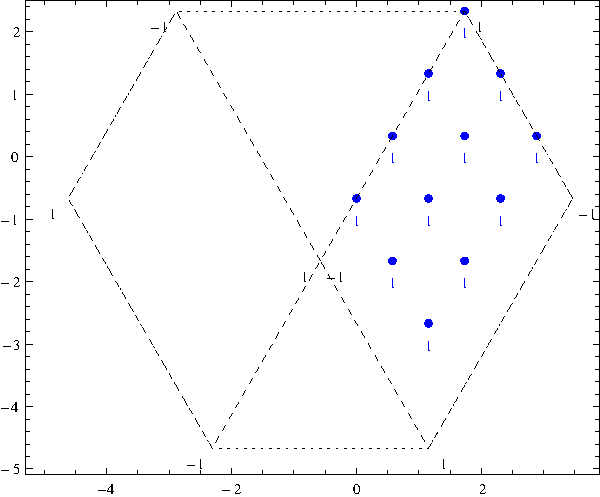
\includegraphics[width=120mm]{a2-a1}
  }
  \caption{Weyl group orbit (dotted) producing singular element of $A_{2}$-module $L^{(3,2)}$ and its decomposition into the sum of splint images of singular elements of $A_{1}\oplus A_{1}$-modules (dashed). Weight multiplicities of $A_{1}\oplus A_{1}$-module coincide with branching coefficients for the reduction $L^{(3,2)}_{A_{2}\downarrow A_{1}\oplus u(1)}$.}

 \label{fig:a2_splint}
\end{figure}
\end{example}
\begin{example}
  Now consider Lie algebra $B_{2} (\bf{so}(5))$ and branching of its irreducible module $L^{(3,2)}$ into the modules of reductive subalgebra $A_{1}\oplus u(1)$ with root system spanned by first simple root of $B_{2}$. Singular element of $L^{(3,2)}$ is decomposed into the sum of splint images of singular elements of $A_{2}$-modules and branching coefficients coincide with weight multiplicities of $A_{2}$-module (see Fig. \ref{fig:b2_splint}).

  \begin{figure}[h!bt]
  \hspace*{-1.5cm}

   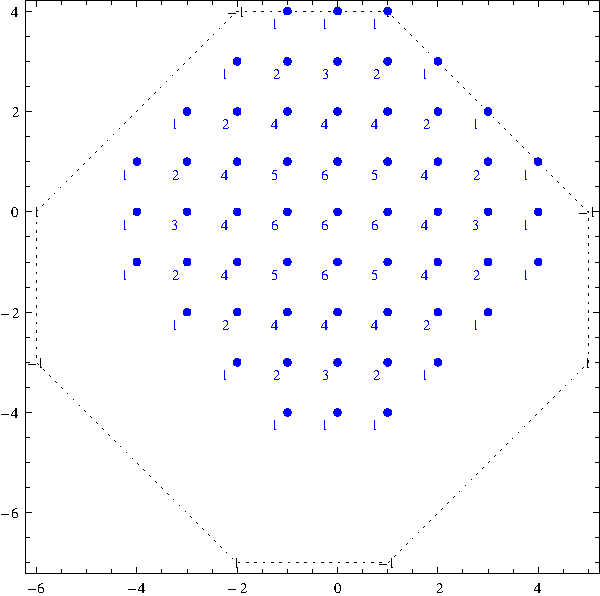
\includegraphics[width=75mm]{b2}
   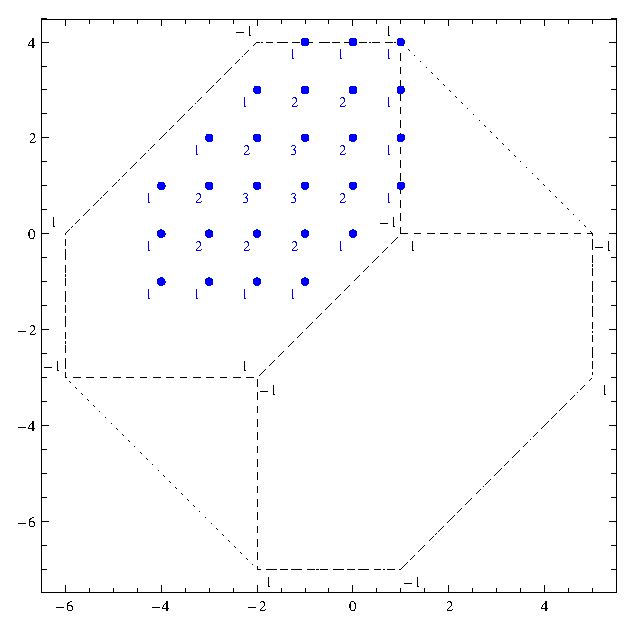
\includegraphics[width=75mm]{b2-a2-a1}
  \caption{$B_{2}$-module $L^{(3,2)}$ is shown on the left. Weight multiplicities are indicated. Contour of singular element is shown by dotted line. Right figure represents the decomposition of  $L^{(3,2)}$-singular element into the sum of splint images of singular elements of $A_{2}$-modules (dashed). Weight multiplicities of $A_{2}$-module coincide with branching coefficients for the reduction $L^{(3,2)}_{B_{2}\downarrow A_{1}\oplus u(1)}$.}

 \label{fig:b2_splint}
\end{figure}
\end{example}
\begin{example}
   Lie algebra $G_{2}$ has regular subalgebra $A_{2}$ with root system built on long roots of $G_{2}$. Consider branching of its irreducible module $L^{(3,2)}$ into the modules of reductive subalgebra $A_{2}$. Singular element of $L^{(3,2)}$ is decomposed into the sum of splint images of singular elements of $A_{2}$-modules and branching coefficients coincide with weight multiplicities of $A_{2}$-module (see Fig. \ref{fig:g2_splint}).


  \begin{figure}[h!bt]
  \noindent\centering{
   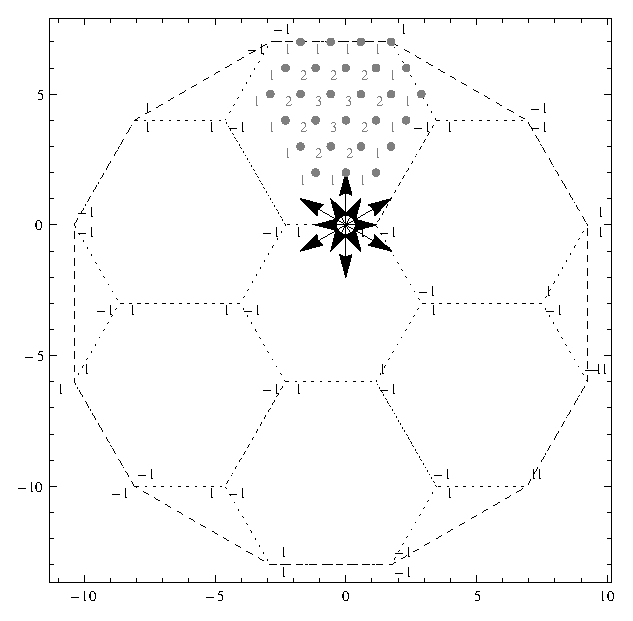
\includegraphics[width=120mm]{g2}
  }

  \caption{Weyl group orbit (dotted) producing singular element of $G_{2}$-module $L^{(3,2)}$ and its decomposition into the sum of splint images of singular elements of $A_{2}$-modules (dashed). Weight multiplicities of $A_{2}$-module coincide with branching coefficients for the reduction $L^{(3,2)}_{G_{2}\downarrow A_{2}}$.}


 \label{fig:g2_splint}
\end{figure}

\end{example}

\section{Conclusions}

\label{sec:conclusions}It is explicitly demonstrated that splint
presents a very effective tool to find branching coefficients. In
particular injective splints provide a possibility to reduce
branching rules calculations for highest weight modules to a
determination of weight multiplicities for a module with the same
Dynkin labels referred to a different Lie algebra. This algebra
$\frak{s}$ must not be a subalgebra in the initial $\frak{g}$ , it
has the same rank $r_{\frak{s}}=r$\ , but as a rule is less
complicated than $\frak{g}$ .

It is significant that for the injections $D_{r}\hookrightarrow B_{r}$ , $%
D_{r}\hookrightarrow C_{r}$ and $A_{r}\hookrightarrow
A_{r-1}\oplus u\left( 1\right) $ splint technique shows
immediately Gelfand-Tzeytlin rules for branching: the nonzero
branching coefficients are equal to 1, the reduction is
multiplicity free. Here it is an immediate consequence of the
structure of the second stem being a direct sum of $A_{1}$
algebras and the fact that the corresponding module
$L_{\frak{s}}^{\mu }$ is irreducible.

\section*{Acknowledgements}
\label{sec:acknowledgements}
The work was supported in part by the
RFFI grant N 09-01-00504. The work of A.A.~Nazarov is supported by
the Chebyshev Laboratory (Department of Mathematics and Mechanics,
Saint-Petersburg State University) under the grant 11.G34.31.0026
of the Government of the Russian Federation.


\bibliography{bibliography}{}
\bibliographystyle{utphys}

%%%%%%%%%%%%%%%%%%%%%%%%%%%%%%%%%%%%%%%%%%%%%%%%%%%%%%%%%%%%%


%%%%%%%%%%%%%%%%%%%%%%%%%%%%%%%%%%%%%%%%%%%%%%%%%%%%%%%%%%%%%
\section*{Appendix}

%%%%%%%%%%%%%%%%%%%%%%%%%%%%%%%%%%%%%%%%%%%%%%%%%%%%%%%%%%%%%

Let us demonstrate that for injective splints of classical Lie
algebras the following property is valid:

Let $\Delta \approx (\Delta _{\frak{a}},\Delta _{\frak{s}})$ be an
injective
splint with the decomposition of simple roots $S=S_{\frak{c}}\cup S_{\frak{d}%
}$ with $S_{\frak{c}}=S\cap S_{\frak{a}}$ and $S_{\frak{d}}=S\cap S_{\frak{s}%
}$.

Then for any simple root $\beta \in S_{\frak{s}}$ there exists the
pair of
roots ( $\alpha $ ,$\beta ^{\prime }$) with $\alpha \in $ $S_{\frak{c}%
},\beta ^{\prime }\in S_{\frak{s}}$ such that $\alpha =\beta
-\beta ^{\prime }$

Type 1. $\Delta _{G_{2}}\approx (\Delta _{A_{2}},\Delta
_{A_{2}}).$

 \begin{figure}[h!bt]
  \noindent\centering{
   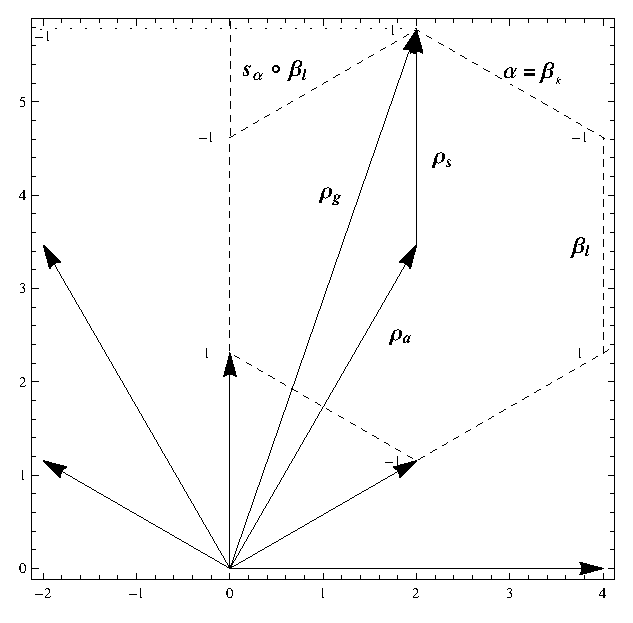
\includegraphics[width=100mm]{g2-roots}
  }
  \caption{Weyl group orbit (dotted) producing singular element of $A_{2}$-module $L^{(3,2)}$ and its decomposition into the sum of splint images of singular elements of $A_{1}\oplus A_{1}$-modules (dashed). Weight multiplicities of $A_{1}\oplus A_{1}$-module coincide with branching coefficients for the reduction $L^{(3,2)}_{A_{2}\downarrow A_{1}\oplus u(1)}$.}
\end{figure}
Here both stems are metric and the corresponding root systems are
equivalent. In Figure 4 a part of the singular element $\Phi
_{G_{2}}^{\left( 0\right) }$ is presented. The boundaries of $\bar{C_{\frak{a%
}}}$ are the dashed lines starting in the center of the singular
element. It
contains the edge $\lambda _{2}=-\alpha _{2}=-\beta _{2}$ and the roots $%
-\beta _{1}=-s_{\alpha _{2}}\circ \beta _{3}$ , $-\beta _{3}$
($\beta _{3}$ is indicated as $\beta _{l}$). For this root $\beta
_{1}$ the necessary pair
is ( $\alpha _{1}$ ,$\beta _{2}$): $\alpha _{1}=\beta _{1}-\beta _{2}$. The $%
\lambda _{2,3}^{\frak{s}}=\beta _{3}$ edge is equal to $\lambda _{1}^{\frak{s%
}}=\beta _{1}=s_{\alpha _{2}}\circ \beta _{3}$ and $m_{1}$ indice
is aquired by the $\frak{s}$-module that inherit the second
indice. In this particular
case they are $m_{1}=m_{2}=0$. The general case with the initial module $%
L^{\mu }$ and $\mu =m_{1}\omega _{1}+m_{2}\omega _{2}$.can be
treated in the same way: one finds an edge $\lambda _{2}=-\left(
m_{2}+1\right) \beta _{2}$ and put $\lambda
_{1}^{\frak{s}}=-\left( m_{1}+1\right) \beta _{1}$, its end
belongs to the boundary $\bar{C_{\frak{a}}}$ . The reflection
$s_{\beta
_{2}} $ sends $\beta _{1}$ to $\beta _{3}$ and the corresponding edge $%
\lambda _{2,3}^{\frak{s}}=-\left( m_{1}+1\right) \beta _{3}$ has
the same length. Now consider $\lambda _{1}^{\frak{s}}$ (or
$\lambda _{2,3}^{\frak{s}} $) and $\lambda _{1,3}^{\frak{s}}$ (or
$\lambda _{2,3,1}^{\frak{s}}$) edges to find that they belong to
the boundary $\bar{C_{\frak{a}}}$ and the Weyl symmetry predicts
that $\lambda _{1,3}^{\frak{s}}=-\left( m_{2}+1\right)
\beta _{3}$ ($\lambda _{2,3,1}^{\frak{s}}=-\left( m_{2}+1\right) \beta _{1}$%
) . Finally the edge $\lambda _{1,3,2}^{\frak{s}}=-\left(
m_{1}+1\right) \beta _{2}$ close the polytop . The latter
corresponds to the singular
element $\Phi _{\frak{s}}^{\left( \widetilde{\mu }\right) }=\sum_{w\in W_{%
\frak{s}}}\varepsilon \left( w\right) e^{w\circ \left(
\widetilde{\mu }+\rho
_{\frak{s}}\right) }$ of the module $L_{\frak{s}}^{\left( \widetilde{\mu }%
\right) }$ with $\widetilde{\mu }=m_{1}\widetilde{\omega }_{1}+m_{2}%
\widetilde{\omega }_{2}$ . Notice that in this case the sign
factors can be obtained directly in the initial weight system as
far as the stem is metric.

Type 1. $\Delta _{F_{4}}\approx (\Delta _{D_{4}},\Delta
_{D_{4}}).$

Both stems are metric and the corresponding root systems are
equivalent. The system $\Delta _{D_{4}}$ of the subalgebra
$\frak{a=}D_{4}$ is formed by the set $\left\{ \pm e_{i},\pm
e_{j}\right\} _{|i,j=1,\ldots 4,\quad i\neq j}$ . The simple roots
$S_{\frak{c}}$ are $\left\{ e_{2}-e_{3},e_{3}-e_{4}\right\} $ and
$S_{\frak{d}}=\left\{ e_{4},\frac{1}{2}\left(
e_{1}-e_{2}-e_{3}-e_{4}\right) \right\} $.

For a module $L^{\mu }$ with $\mu =\sum m_{k}\omega _{k}$ consider the edge $%
\lambda _{3}=-\left( m_{3}+1\right) e_{4}=-\left( m_{3}+1\right)
\beta _{3}$
\ Compose an edge $\lambda _{2}^{\frak{s}}=-\left( \widetilde{m}%
_{2}+1\right) \beta _{2}$ . Now the necessary pair is $\left(
\alpha
_{2}=e_{3}-e_{4},\beta _{3}\right) $. The intersection of $\lambda _{2}^{%
\frak{s}}$ with the $\alpha _{2}$ -boundary of
$\bar{C_{\frak{a}}}$ fixes
its length to be $\lambda _{2}^{\frak{s}}=-\left( m_{2}+1\right) \beta _{2}$%
\ and the length of the edge $\lambda _{3,2}^{\frak{s}}$ is equal
to that of
$\lambda _{2}^{\frak{s}}$. Next consider the edge $\lambda _{2}^{\frak{s}%
}=-\left( m_{2}+1\right) \beta _{2}$ and the pair $\left( \alpha
_{1}=e_{2}-e_{3},\beta _{1}=e_{2}\right) $ \ The length of the
edge $\lambda _{1}^{\frak{s}}$ becomes equal to $\lambda
_{1}^{\frak{s}}=-\left( m_{1}+1\right) \beta _{1}$ and so on. The
edges along the roots like $\alpha _{4}=\beta
_{4}=\frac{1}{2}\left( e_{1}-e_{2}-e_{3}-e_{4}\right) $ are
treated similarly and finally the singular element $\Phi
_{\frak{s}}^{\left( \widetilde{\mu }\right) }=\sum_{w\in
W_{\frak{s}}}\varepsilon \left( w\right) e^{w\circ \left(
\widetilde{\mu }+\rho _{\frak{s}}\right) }$ of the module
$L_{\frak{s}}^{\left( \widetilde{\mu }\right) }$ with
$\widetilde{\mu }=\sum m_{k}\widetilde{\omega }_{k}$ is formed in
$\bar{C_{\frak{a}}}$.

Type 2. $\Delta _{B_{r}}\approx (\Delta _{D_{r}},\Delta _{\oplus
^{r}A_{1}}). $

Both stems are metric. The injection is fixed by the stem $\Delta
_{D_{r}}$ with simple roots $S_{\frak{a}}=\left\{
e_{1}-e_{2},e_{2}-e_{3},\ldots
,e_{r-1}-e_{r},e_{r-1}+e_{r}\right\} $ . The second stem
corresponds to a
direct sum of algebras $A_{1}$ and has the simple roots $S_{\frak{s}%
}=\left\{ e_{1},e_{2},\ldots ,e_{r-1},e_{r}\right\} $. Consider the edge $%
\lambda _{r}=-\left( m_{r}+1\right) \beta _{r}$ (here $\beta
_{r}=e_{r}$) and .$\lambda _{r-1}=-\left(
\widetilde{m}_{r-1}+1\right) \beta _{r-1}$
attached to it (here $\beta _{r-1}=e_{r-1}$). The corresponding pair is $%
\left( \alpha _{r-1}=e_{r-1}-e_{r},\beta _{r-1}=e_{r-1}\right) $
.\ The intersection condition fixes the second edge to be $\lambda
_{r-1}=-\left( m_{r-1}+1\right) \beta _{r-1}$ , it is orthogonal
to $\beta _{r}$ so the opposite edge has the same length. The
Dynkin indice $m_{r-1}$ now refers
also to the\ simple root $\beta _{r-1}$ . Next consider the obtained edge $%
\lambda _{r-1}=-\left( m_{r-1}+1\right) \beta _{r-1}$ and $\lambda
_{r-2}=-\left( \widetilde{m}_{r-2}+1\right) \beta _{r-2}$ to
obtain the indice $\widetilde{m}_{r-2}=m_{r-2}$ and the edge
$\lambda _{r-2}=-\left( m_{r-2}+1\right) \beta _{r-2}$ and so on
till all the pairs of edges are properly fixed. Finally in
$\bar{C_{D_{r}}}$ the element $\Phi _{\oplus ^{r}A_{1}}^{\left(
\widetilde{\mu }\right) }=\sum_{w\in W_{\oplus
^{r}A_{1}}}\varepsilon \left( w\right) e^{w\circ \left( \widetilde{\mu }+%
\frac{1}{2}\sum e_{k}\right) }$ can be constructed for the module
$L_{\oplus ^{r}A_{1}}^{\left( \widetilde{\mu }\right) }$ with
$\widetilde{\mu }=\sum m_{k}\frac{1}{2}e_{k}$ .

Type 2. $\Delta _{C_{r}}\approx (\Delta _{D_{r}},\Delta _{\oplus
^{r}A_{1}}). $

The situation in this case is eqivalent to the previous one and
the additional edges are constructed similarly.

Type 3 $\Delta _{A_{r}}\approx (\Delta _{A_{r-1}\oplus
u_{1}},\Delta _{\oplus ^{r}A_{1}}).$

Here only the first stem is metric and it fixes the injection with
simple roots $S_{\frak{a}}=\left\{ e_{1}-e_{2},e_{2}-e_{3},\ldots
,e_{r-1}-e_{r}\right\} $ . The second stem corresponding to a direct sum of $%
r$ copies of $A_{1}$ has the simple roots $S_{\frak{s}}=\left\{
e_{1}-e_{r+1},e_{2}-e_{r+1},\ldots ,e_{r}-e_{r+1}\right\} $.
Consider the edge $\lambda _{r}=-\left( m_{r}+1\right) \beta _{r}$
with $\beta
_{r}=e_{r}-e_{r+1}$ and .$\lambda _{r-1}=-\left( \widetilde{m}%
_{r-1}+1\right) \beta _{r-1}$ \ with $\beta
_{r-1}=e_{r-1}-e_{r+1}$ attached to it . Then the corresponding
pair is $\left( \alpha _{r-1}=e_{r-1}-e_{r},\beta
_{r-1}=e_{r-1}-e_{r+1}\right) $ .\ The intersection with the
boundary of $\bar{C_{A_{r-1}}}$ orthogonal to $\alpha _{r-1}$
fixes the second edge to be $\lambda _{r-1}=-\left(
m_{r-1}+1\right) \beta _{r-1}$. The Dynkin indice $m_{r-1}$ is to
be used for the fundamental weight  $\omega _{r-1}$ . The\
reflection $s_{\beta _{r}}$ sends $\lambda _{r-1}=-\left(
m_{r-1}+1\right) \beta _{r-1}$ to $\lambda _{r,r-1}=-\left(
m_{r-1}+1\right) \beta _{r-1}$\ . Next consider the obtained edge
$\lambda _{r-1}=-\left( m_{r-1}+1\right) \beta _{r-1}$ and
$\lambda _{r-2}=-\left( \widetilde{m}_{r-2}+1\right) \beta _{r-2}$
with $\beta _{r-2}=e_{r-2}-e_{r+1} $ to obtain the indice
$\widetilde{m}_{r-2}=m_{r-2}$ and the edge $\lambda _{r-2}=-\left(
m_{r-2}+1\right) \beta _{r-2}$ and so on till all the pairs of
edges are properly fixed. Finally in $\bar{C_{D_{r}}}$ the element
$\Phi _{\oplus ^{r}A_{1}}^{\left( \widetilde{\mu }\right)
}=\sum_{w\in W_{\oplus
^{r}A_{1}}}\varepsilon \left( w\right) e^{w\circ \left( \widetilde{\mu }+%
\widetilde{\rho }\right) }$ can be constructed for the module
$L_{\oplus ^{r}A_{1}}^{\left( \widetilde{\mu }\right) }$ with
$\widetilde{\mu }=\sum m_{k}\beta _{k}$ . The simplest case
$\Delta _{A_{2}}\approx (\Delta _{A_{1}\oplus u_{1}},\Delta
_{A_{1}\oplus A_{1}})$ is presented in Example 4.1 and Figure 1.

Type 3 $\Delta _{B_{2}}\approx (\Delta _{A_{1}},\Delta _{A_{2}}).$

The necessary elements are presented in Example 4.1 and Figure 1 , $%
S_{A\_1}=\left\{ e_{1}-e_{2}\right\} $ , $S_{A\_2}=\left\{
e_{1},e_{2}\right\} $.The edge $\lambda _{\alpha _{2}}=\lambda
_{\beta _{2}}=-\left( m_{2}+1\right) \beta _{2}$ has an edge
$\lambda _{\beta _{1}}=-\left( \widetilde{m}_{1}+1\right) \beta
_{1}$ attached to it. Consider the pair $\left( \alpha
_{1}=e_{1}-e_{2},\beta _{1}=e_{1}\right) $ .The end of the edge
$\lambda _{\beta _{1}}$ is to define a weight
invariant under the reflexion $s_{\alpha _{1}}$ . This defines its length: $%
\lambda _{\beta _{1}}=-\left( m_{1}+1\right) \beta _{1}$ . In the
coimage of
the second stem, that is in the $A_{2}$ root system, the reflection $%
s_{\beta _{2}}$ sends $\lambda _{\beta _{1}}=-\left(
m_{1}+1\right) \beta
_{1}$ to $\lambda _{2,3}$\ ., thus the latter edge has the same length in $%
\beta _{3}=e_{1}+e_{3}$ , we have $\lambda _{2,3}=-\left(
m_{1}+1\right)
\beta _{3}$ with $\beta _{3}=e_{1}+e_{3}$ . The irreducible $\frak{s}$%
-module has the highest weight $\widetilde{\mu }=m_{1}\widetilde{\omega }%
_{1}+m_{2}\widetilde{\omega }_{2}$ . In Figure 1 we see the
details of these relations in a particular case where
$L_{B_{2}}^{\left[ 3,2\right] }$ is reduced to a subalgebra
$A_{1}\oplus u\left( 1\right) $ and the
corresponding highest weights with their multiplicities form the diagram $%
\mathcal{N}_{A\_2}^{\left[ 3,2\right] }$ .


%%%%%%%%%%%%%%%%%%%%%%%%%%%%%%%%%%%%%%%%%%%%%%%%%%%%%%%%%%%%%
%%%%%%%%%%%%%%%%%%%%%%%%%%%%%%%%%%%%%%%%%%%%%%%%%%%%%%%%%%%%%

\end{document}
